\documentclass[a4paper]{article}
\usepackage[margin=0.65in]{geometry}
\usepackage{times}
\usepackage{pgfplots}
\pgfplotsset{compat=1.18}
\pagestyle{empty}
\begin{document}
\begin{center}{\Large\bfseries Task 4: OpenMP scheduling}\\[5pt]
$N=256$, $t_{\mathrm{end}}=100$, $\Delta t=0.01$; median of 3 runs on Euler.\\
All three panels use linear axes and identical limits.\end{center}
\begin{center}
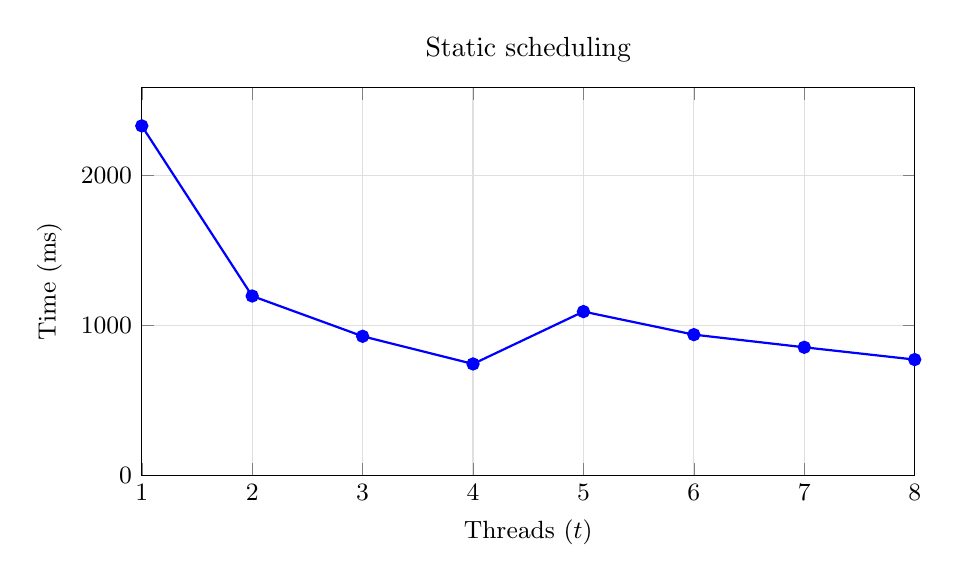
\begin{tikzpicture}
\begin{axis}[width=0.94\linewidth,height=6.5cm,
title={Static scheduling},xlabel={Threads ($t$)},ylabel={Time (ms)},
xmin=1,xmax=8,ymin=0,ymax=2585.23267464,xtick={1,2,3,4,5,6,7,8},
grid=major,major grid style={gray!25},scaled y ticks=false,
tick label style={font=\small},label style={font=\small},
/pgf/number format/1000 sep={}]
\addplot[blue,thick,mark=*,mark size=2pt] coordinates {
(1, 2331.569239)
(2, 1195.889727)
(3, 927.038424)
(4, 742.311509)
(5, 1091.908749)
(6, 938.0144)
(7, 853.580674)
(8, 771.527754)
};
\end{axis}
\end{tikzpicture}
\end{center}
\begin{center}
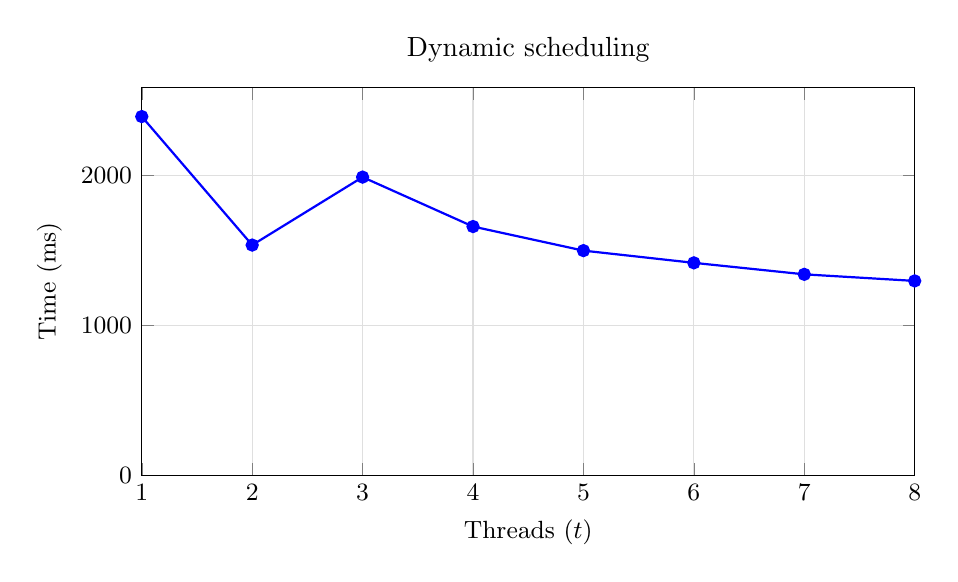
\begin{tikzpicture}
\begin{axis}[width=0.94\linewidth,height=6.5cm,
title={Dynamic scheduling},xlabel={Threads ($t$)},ylabel={Time (ms)},
xmin=1,xmax=8,ymin=0,ymax=2585.23267464,xtick={1,2,3,4,5,6,7,8},
grid=major,major grid style={gray!25},scaled y ticks=false,
tick label style={font=\small},label style={font=\small},
/pgf/number format/1000 sep={}]
\addplot[blue,thick,mark=*,mark size=2pt] coordinates {
(1, 2393.733958)
(2, 1535.909613)
(3, 1989.561264)
(4, 1659.57706)
(5, 1498.833492)
(6, 1417.277686)
(7, 1340.544556)
(8, 1296.621878)
};
\end{axis}
\end{tikzpicture}
\end{center}
\begin{center}
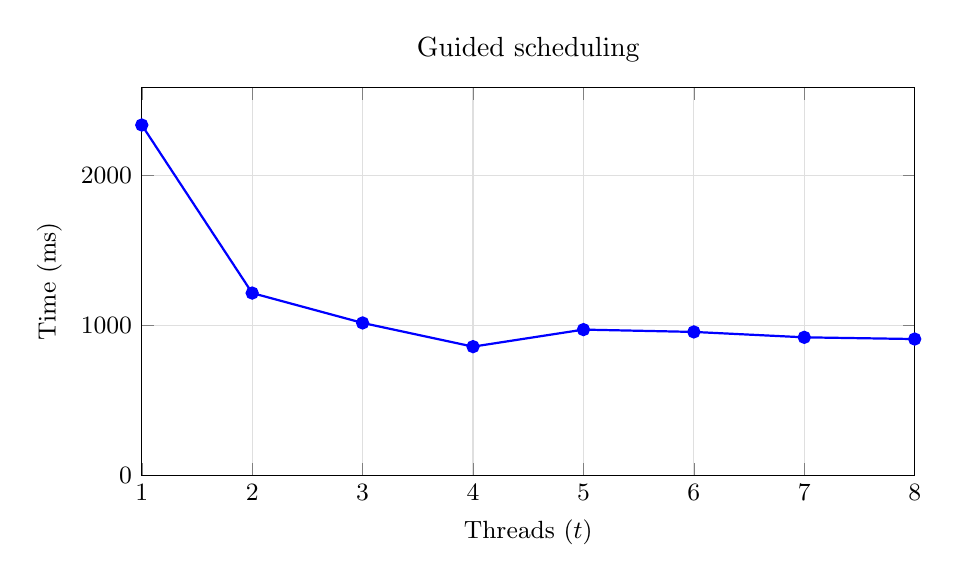
\begin{tikzpicture}
\begin{axis}[width=0.94\linewidth,height=6.5cm,
title={Guided scheduling},xlabel={Threads ($t$)},ylabel={Time (ms)},
xmin=1,xmax=8,ymin=0,ymax=2585.23267464,xtick={1,2,3,4,5,6,7,8},
grid=major,major grid style={gray!25},scaled y ticks=false,
tick label style={font=\small},label style={font=\small},
/pgf/number format/1000 sep={}]
\addplot[blue,thick,mark=*,mark size=2pt] coordinates {
(1, 2337.318849)
(2, 1215.536533)
(3, 1016.097363)
(4, 857.847123)
(5, 971.613289)
(6, 956.106722)
(7, 920.07939)
(8, 908.582073)
};
\end{axis}
\end{tikzpicture}
\end{center}
\end{document}
